% ========== FASAN ==========
\begin{frame}{%
  \begin{minipage}[c]{0.30\textwidth}
    Fasan
  \end{minipage}%
  \hfill
  \begin{minipage}[c]{0.45\textwidth}
    \footnotesize
    \textbf{Jagttid:} 1.\ oktober -- 31.\ januar
  \end{minipage}%
  \hfill
  \begin{minipage}[c]{0.15\textwidth}
    \noindent\raggedleft
    
\includegraphics[width=0.5cm, height=0.5cm, keepaspectratio]{Billeder/Ikoner/star.png}%
    \hspace{0.2em}%
    
\includegraphics[width=0.5cm, height=0.5cm, keepaspectratio]{Billeder/Ikoner/star.png}%
    \hspace{0.2em}%
    
\includegraphics[width=0.5cm, height=0.5cm, keepaspectratio]{Billeder/Ikoner/star.png}
  \end{minipage}%
}
  \vspace{0.25em}
  \begin{columns}[T]
    % --- Venstre kolonne: Tekst ---
    \column{0.45\textwidth}
    \setlength{\parskip}{0.5em}
    \tiny
    \RaggedRight
    \textbf{\textit{Phasianus colchicus}} – stor hønsefugl med lang hale \par
    \textbf{Udseende:}\\
    \quad – Kok: Kobberrød krop, grønt hoved, røde kindpletter, ofte hvid halsring \\
    \quad – Høne: Brunspraglet, mere camoufleret, kortere hale \par
    \textbf{Levesteder:} Marker, læhegn, småskove og moser. \par
    \textbf{Føde:} Frø, korn, bær, insekter og snegle. \par
    \textbf{Udbredelse:} Hele Danmark. \par
    \textbf{Træk/standfugl:} Standfugl \par
    \textbf{Forplantning:}\\
    \quad – \textbf{Yngleforhold:} Yngler i hele Danmark \\
    \quad – \textbf{Kønsmoden:} Ca. 1 år \\
    \quad – \textbf{Mono/polygam:} Polygam \\
    \quad – \textbf{Bestandsomsætning:} Hurtig \\
    \quad – \textbf{Kuld:} 8–15 æg
    % --- Højre kolonne: To billeder ---
    \column{0.52\textwidth}
    \centering
    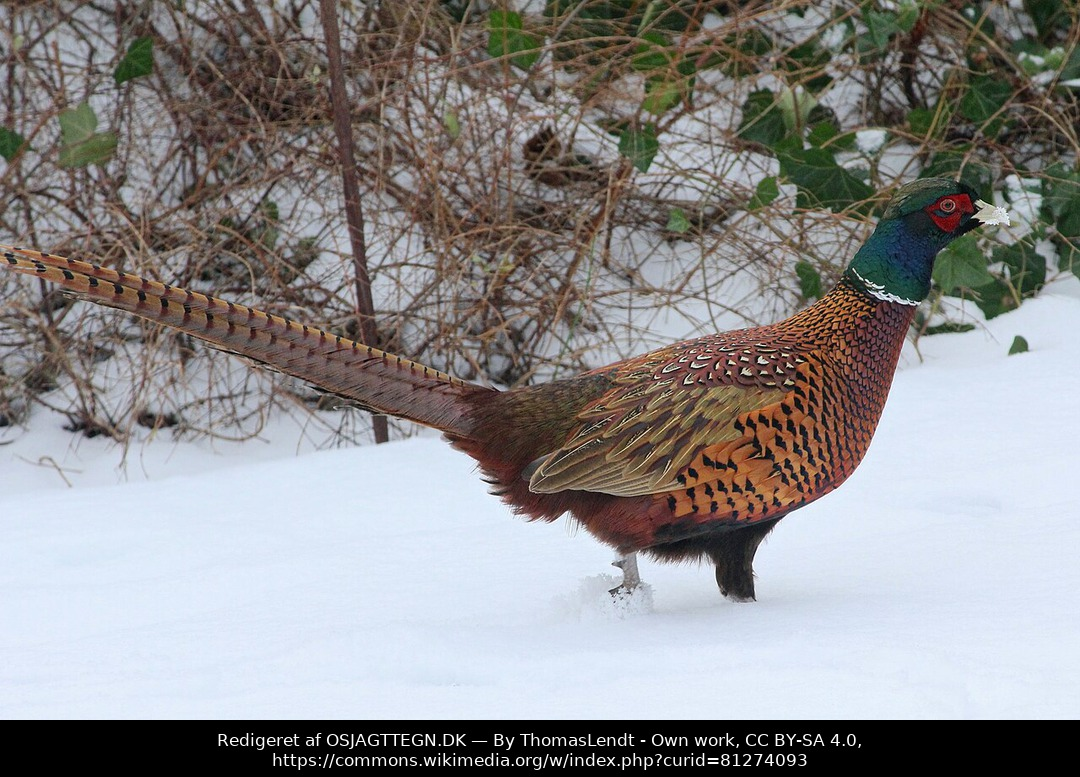
\includegraphics[width=0.92\linewidth, height=3cm, keepaspectratio]{Billeder/Dyr/Fugle/Fasanfugle/Fasan/fasan-male-01.jpg}\\[0.45em]
    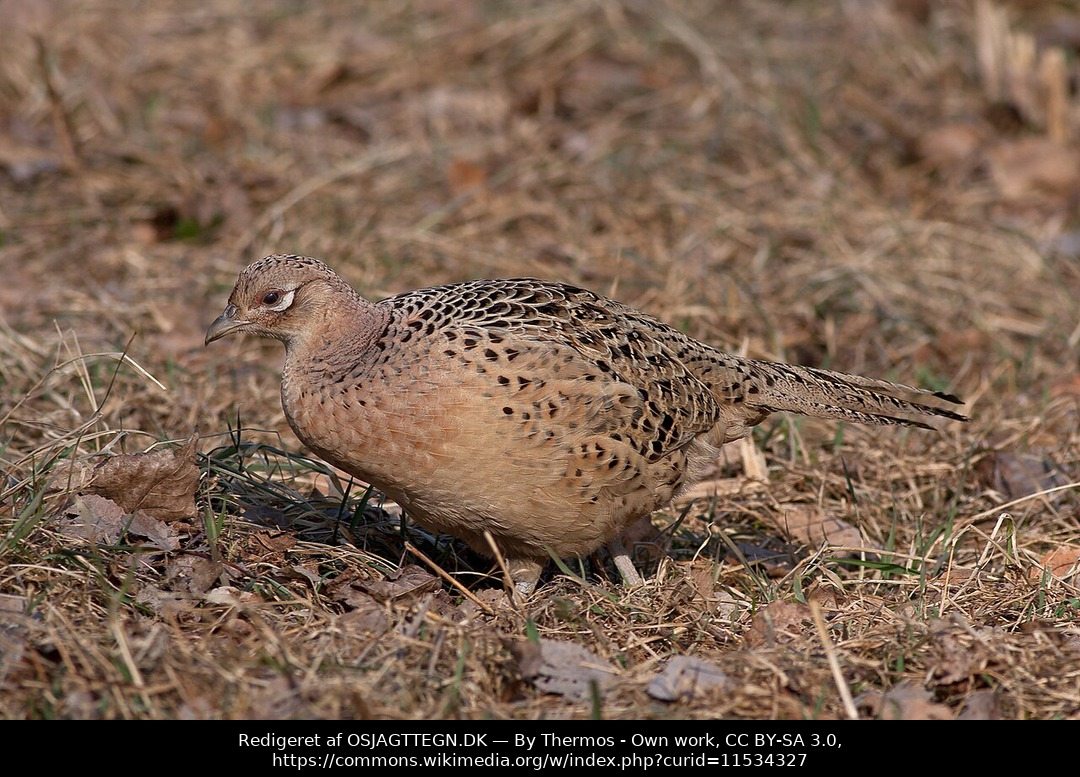
\includegraphics[width=0.92\linewidth, height=3cm, keepaspectratio]{Billeder/Dyr/Fugle/Fasanfugle/Fasan/fasan-female-01.jpg}\\[0.25em]
    \footnotesize Kok øverst, høne nederst
  \end{columns}
\end{frame}